\documentclass{article}
\usepackage[T1]{fontenc}
\usepackage[utf8]{inputenc}
\usepackage[portuguese]{babel}

\title{Lista 2 \\
\large Equações Diferenciais Parciais \\
Difusão de calor em um \textit{grid}}
\author{Lucas Emanuel Resck Domingues}
\date{Setembro de 2020}

\usepackage{natbib}
\usepackage{graphicx}
\usepackage{amsmath}
\usepackage{hyperref}
\usepackage{listings}

%Hyperlinks
\usepackage{hyperref}
\hypersetup{
    colorlinks=true,
    allcolors=,  % Nothing change colors
    urlcolor=blue  % URL changes color
}

\begin{document}

    \maketitle
    
    \section*{No papel}

        Consideremos a equação da difusão nos vértices do grafo:
        \begin{alignat*}{2}
            u_t =& -cLu \\
            =& c(A-D)u \\
            =&c[u(x+\Delta x, y)-u(x, y) \\
            &+u(x-\Delta x, y)-u(x, y) \\
            &+u(x, y+\Delta y)-u(x, y) \\
            &+u(x, y-\Delta y)-u(x, y)] \\
        \end{alignat*}
        Consideremos a expressão da derivada parcial de segunda ordem
        de $u$ em relação a $x$, porém sem o limite:
        $$\hat{u}_{xx}(x, y) = \dfrac{u_x(x + \Delta x, y) - u_x(x, y)}{\Delta x}$$
        Para a de primeira ordem:
        $$\hat{u}_{x}(x, y) = \dfrac{u(x, y) - u(x - \Delta x, y)}{\Delta x}$$
        Voltando para a de segunda ordem, escrevemos então $\widetilde{u}_{xx}$:
        $$\widetilde{u}_{xx} = \dfrac{u(x+\Delta x, y)-2u(x, y)+u(x-\Delta x, y)}{(\Delta x)^2}$$
        Fazemos para $y$ de maneira análoga. Então temos:
        $$u_t = c[(\Delta x)^2\widetilde{u}_{xx} + (\Delta y)^2\widetilde{u}_{yy}]$$
        Assumindo que o limite exista, podemos tomar $\Delta x = \Delta y$ e tomar o limite:
        \begin{align*}
            u_t &= \widetilde{c}(u_{xx} + {u_{yy}}) \\
            &= \widetilde{c} \Delta u
        \end{align*}

    \section*{Computacional}

        O código foi escrito em \textit{Python} e utilizou as bibliotecas \textit{Numpy}, \textit{Matplotlib} e \textit{Seaborn}. Ele pode ser conferido no Apêndice \ref{appendix:a}.

        As simulações constam de um \textit{grid} 32 por 32 com calor constante nos bordos do sistema.
        A dispersão do calor é calculada utilizando a equação de difusão do calor em \textit{grid}.

        Um \textit{grid} é representado por um array 32 por 32. A atualização do \textit{grid} ocorre até que 
        duas iterações consecutivas estejam próximas por uma tolerância de $10^{-2}$, na norma de Frobenius.

        \begin{itemize}
            \item[(a)] Para a primeira difusão, com temperatura 10 constante nos bordos do \textit{grid}
                e $c=0.1$, foram necessárias 1921 iterações para a convergência com tolerância $10^{-2}$. Visualizamos algumas das etapas da difusão na Figura \ref{fig:graph_1}.
                
                \begin{figure}[!h]
                    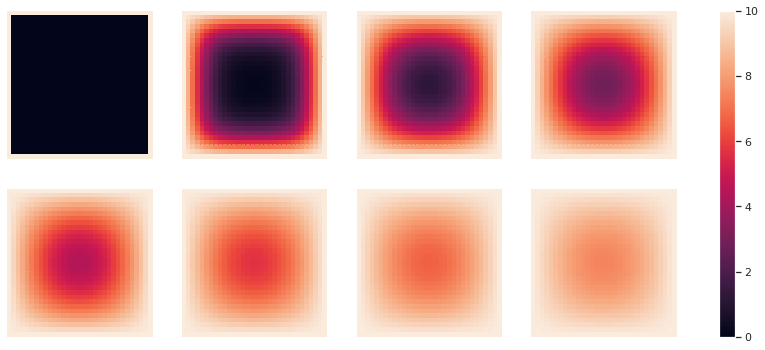
\includegraphics[width=\textwidth]{graph_1.png}
                    \caption{Gráficos de difusão do calor em um \textit{grid} 32 por 32, com temperatura constante 10 nos bordos.}
                    \label{fig:graph_1}
                \end{figure}

                Observamos que o \textit{grid} aparenta convergir para uma temperatura constante de 10 em todos os vértices.
                Isso é plausível, afinal está sendo inserido calor no sistema (temperatura constante nos bordos, por mais que haja difusão
                para dentro do \textit{grid}.)

            \item[(b)] Para a segunda simulação, os bordos horizontais têm temperatura constante de 10,
                enquanto os verticais, 20. Para $c=0.1$, foram necessárias 2118 iterações até a convergência. Algumas etapas da simulação
                podem ser conferidas na Figura \ref{fig:graph_2}.
                
                \begin{figure}[!h]
                    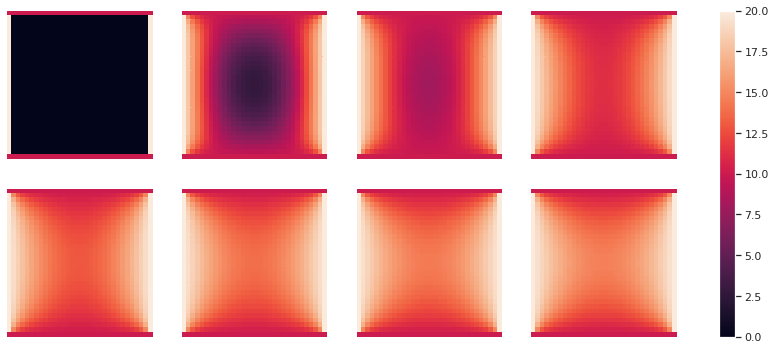
\includegraphics[width=\textwidth]{graph_2.png}
                    \caption{Gráficos de difusão do calor em um \textit{grid} 32 por 32, com temperaturas constantes, porém diferentes, nos bordos.}
                    \label{fig:graph_2}
                \end{figure}

                Observamos que o sistema converge para um sistema aparentemente simétrico, com um efeito gradiente ao se mover
                de um bordo horizontal para um vertical. Compreensível, afinal possuem bordos com temperaturas constantes porém diferentes.

                A temperatura de equilíbro depende da posição do vértice no gráfico, mais especificamente das distâncias em relação aos bordos.
                Por exemplo, observamos que os vértices centrais possuem temperatura próxima a 15, o que é intuitivo dado que é a média de 10 e 20
                e o sistema apresenta simetria.

        \end{itemize}

    \newpage

    \appendix

    \section{Código para a difusão de calor em \textit{grid}}
        \label{appendix:a}

        O código também pode ser conferido \href{https://github.com/lucasresck/pde/blob/master/list_2/list_2.ipynb}{neste \textit{notebook} no \textit{GitHub}}.

        \begin{lstlisting}[language=Python]
def make_grid(n, t_min, t_max_v, t_max_h):
    """Make the graph."""
    grid = np.zeros((n, n))
    grid[:, :] = t_min
    grid[:, 0] = t_max_v
    grid[:, n-1] = t_max_v
    grid[0, :] = t_max_h
    grid[n-1, :] = t_max_h
    return grid

def plot_grid(grid, ax, vmin=0, vmax=10):
    """Plot the temperatures of the grid."""
    sns.heatmap(grid, vmin=vmin, vmax=vmax,
                ax=ax, cbar=False)
    ax.set_xticks(ticks=[])
    ax.set_yticks(ticks=[])

def one_step(grid, c):
    """Calculate next step of the temperatures
    of the grid using graph diffusion equation."""
    grid = grid.copy()
    grid_old = grid.copy()
    n = grid.shape[0]
    for i in range(1, n-1):
        for j in range(1, n-1):
            grid[i, j] += c*(grid_old[i+1, j]
                             + grid_old[i-1, j]
                             + grid_old[i, j+1]
                             + grid_old[i, j-1]
                             - 4*grid[i, j])
    return grid

def whole_process(
    c=0.1, n=32, t_min=0,
    t_max_v=10, t_max_h=10, tol=10**(-2)
):
    
    grid = make_grid(
        n=n, t_min=t_min, t_max_v=t_max_v,
        t_max_h=t_max_h
    )
    
    grids = [grid]
    diff = 1
    while diff > tol:
        grid = one_step(grid, c)
        grids.append(grid)
        diff = np.linalg.norm(grids[-1] - grids[-2], ord='fro')
    
    fig, axes = plt.subplots(2, 4, figsize=(15, 6))

    indices = list(np.linspace(0, len(grids)-1, num=8,
                                endpoint=True, dtype=np.int))
    for j, i in enumerate(indices):
        plot_grid(
            grids[i],
            axes.reshape(-1)[j],
            vmin=t_min,
            vmax=max([t_max_h, t_max_v])
        )
            
    fig.colorbar(
        axes[0, 0].collections[0],
        ax=axes.ravel().tolist()
    )
    
    plt.show()
    
    print('{} steps with tolerance {}.'.format(len(grids), tol))
    return grids
        \end{lstlisting}

\end{document}